\documentclass[letterpaper]{article}
\usepackage[left=2.5cm,top=3cm,right=2.5cm,bottom=3cm,bindingoffset=0.0cm]{geometry}
\usepackage{fontspec}
\usepackage[table]{xcolor}
\usepackage{tabularray}
\usepackage{multicol}
\usepackage{subcaption}
\usepackage{graphicx}

\providefontfamily\samplefont{Scriven}
\providefontfamily\othersamplefont{DejaVu Sans}

\newcommand{\samplefigure}[1]{{\fontsize{48}{48}\samplefont#1}}
\newcommand{\samplefigureother}[1]{{\fontsize{48}{48}\othersamplefont#1}}
\newcommand{\sampleglyph}[1]{{\samplefont\huge#1}}
\newcommand{\sampletext}[1]{{\samplefont\Large#1}}
\newcommand{\sampletextother}[1]{{\othersamplefont\Large#1}}
\newcommand{\codepoint}[1]{{\tt\textcolor{gray}{U+}#1}}
\newcommand{\glyphname}[1]{{\tt#1}}
\newcommand{\glyphref}[2]{\glyphname{#1} (\codepoint{#2})}

\author{Kevin Smith}

\begin{document}

\title{Ophidian}
\maketitle

\section{The Ophidian Writing System}

The Ophidian writing system appeared in the video game \textit{Ultima VII Part Two: Serpent Isle} by Origin Systems.  It is a simple cipher of Latin script and base 10 numerals used in the game to write English.  Each character in Ophidian is composed of curved lines either alone or in joined pairs.  Words in Ophidian are separated by normal spaces and there are also characters for a comma and full stop, although theses are only shown in in-game text, not in any of the supporting documentation.  There is no other punctuation.

In addition to the characters for writing, there are also Ophidian symbols for the philisophical concepts of Chaos, Order, and the Ballance between them.

\section{Updates From Previous Version}

The previous version of this encoding did not specify how combining characters in a pair should be positioned and this ambiguity has been resolved.  This update also adds punctuation and the philisophical serpent symbols.

\section{Style}

In game text usually represents Ophidian as constant width with rounded ends, similar to many ``comic book'' or ``marker'' fonts but it seems like this may have been at least in part due to the limited resolution of video game graphics in 1993.  Variable width fonts with serifs, nib pen, or brushed appearance would be reasonable.  Combined pairs should be treated as a single character when adjusting character spacing. For highly stylized representations like fonts intended for drop caps, snakes or contrast between fire/chaos and ice/order would be particularly appropriate themes.

For the Earth, Chaos, and Order Serpent symbols, the important qualities are that the Chaos serpent is facing toward the Left, the Order serpent is facing toward the right, and the Earth serpent is facing straight up.  The Chaos and Order serpents should also have their heads past the centre line so they are facing away from it instead of towards it as in \glyphref{CADUCEUS}{2624} or some representations of \glyphref{STAFF OF ASCLEPIUS}{2695}.  The number of undulations and the position of the tail are not significant.  If presented as colour emoji, the Earth Serpent should be gold, the Chaos Serpent red or on fire, and the Order Serpent blue or made of ice.

\begin{figure}
  \begin{subfigure}{15em}
    \centering
    \caption{Ballance}
    \samplefigure{\char"E5FB\char"200D\char"E5FA\char"200D\char"E5FC}
  \end{subfigure}
  \begin{subfigure}{15em}
    \centering
    \caption{Caduceus}
    \samplefigureother{\char"2624}
  \end{subfigure}
  \begin{subfigure}{15em}
    \centering
    \caption{Staff of Asclepius}
    \samplefigureother{\char"2695}
  \end{subfigure}
\end{figure}


\section{Code Tables}

\begin{table}
  \caption{Code tables}
  \begin{subtable}[t]{0.7\textwidth}
    \centering
  \caption{Names}\label{names}
  \begin{tblr}{
      column{1} = {cmd={\codepoint}},
      rows = {rowsep=1pt}
    }
    E5E0 & \glyphname{OPHIDIAN SNAKE} \\
    E5E1 & \glyphname{OPHIDIAN CONJOINING SNAKE} \\
    E5E2 & \glyphname{OPHIDIAN REVERSED SNAKE} \\
    E5E3 & \glyphname{OPHIDIAN CONJOINING REVERSED SNAKE} \\
    E5E4 & \glyphname{OPHIDIAN LAZY SNAKE} \\
    E5E5 & \glyphname{OPHIDIAN CONJOINING LAZY SNAKE} \\
    E5E6 & \glyphname{OPHIDIAN REVERSED LAZY SNAKE} \\
    E5E7 & \glyphname{OPHIDIAN CONJOINING REVERSED LAZY SNAKE} \\
    E5E8 & \glyphname{OPHIDIAN TILTED SNAKE} \\
    E5E9 & \glyphname{OPHIDIAN CONJOINING TILTED SNAKE} \\
    E5EA & \glyphname{OPHIDIAN REVERSED TILTED SNAK} \\
    E5EB & \glyphname{OPHIDIAN CONJOINING REVERSED TILTED SNAKE} \\
    E5EC & \glyphname{OPHIDIAN LAZY TILTED SNAKE} \\
    E5ED & \glyphname{OPHIDIAN CONJOINING LAZY TILTED SNAKE} \\
    E5EE & \glyphname{OPHIDIAN REVERSED LAZY TILTED SNAKE} \\
    E5EF & \glyphname{OPHIDIAN CONJOINING REVERSED LAZY TILTED SNAKE} \\
    E5F0 & \glyphname{OPHIDIAN DOUBLE SNAKE} \\
    E5F1 & \glyphname{OPHIDIAN REVERSED DOUBLE SNAKE} \\
    E5F2 & \glyphname{OPHIDIAN HOOK} \\
    E5F3 & \glyphname{OPHIDIAN CONJOINING HOOK} \\
    E5F4 & \glyphname{OPHIDIAN REVERSED HOOK} \\
    E5F5 & \glyphname{OPHIDIAN CONJOINING REVERSED HOOK} \\
    E5F6 & \glyphname{OPHIDIAN LAZY HOOK} \\
    E5F7 & \glyphname{OPHIDIAN CONJOINING LAZY HOOK} \\
    E5F8 & \glyphname{OPHIDIAN REVERSED LAZY HOOK} \\
    E5F9 & \glyphname{OPHIDIAN CONJOINING REVERSED LAZY HOOK} \\
    E5FA & \glyphname{OPHIDIAN EARTH SERPENT} \\
    E5FB & \glyphname{OPHIDIAN CHAOS SERPENT} \\
    E5FC & \glyphname{OPHIDIAN ORDER SERPENT} \\
    E5FD & \textcolor{gray}{\tt(This position shall not be used)} \\
    E5FE & \glyphname{OPHIDIAN COMMA} \\
    E5FF & \glyphname{OPHIDIAN FULL STOP} \\
  \end{tblr}
\end{subtable}
  \begin{subtable}[t]{0.3\textwidth}
    \centering
  \caption{Glyphs}\label{glyphs}
  \begin{tblr}{
      hlines, vlines,
      rows = { halign = c, valign = m, ht = 20pt},
      row{1} = {cmd={\tt}},
      column{1} = {cmd={\tt}},
      cell{2-17}{2-3} = {cmd={\sampleglyph}},
      cell{15}{3} = {bg = gray}
    }
    & E5E & E5F\\
    0 & \char"E5E0 & \char"E5F0 \\
    1 & \char"E5E1\char"25CC & \char"E5F1 \\
    2 & \char"E5E2 & \char"E5F2\\
    3 & \char"E5E3\char"25CC & \char"E5F3\char"25CC\\
    4 & \char"E5E4 & \char"E5F4\\
    5 & \char"E5E5\char"25CC & \char"E5F5\char"25CC\\
    6 & \char"E5E6 & \char"E5F6\\
    7 & \char"E5E7\char"25CC & \char"E5F7\char"25CC\\
    8 & \char"E5E8 & \char"E5F8\\
    9 & \char"E5E9\char"25CC & \char"E5F9\char"25CC\\
    A & \char"E5EA & \char"E5FA\\
    B & \char"E5EB\char"25CC & \char"E5FB\\
    C & \char"E5EC & \char"E5FC\\
    D & \char"E5ED\char"25CC & \\
    E & \char"E5EE & \char"E5FE\\
    F & \char"E5EF\char"25CC & \char"E5FF\\
  \end{tblr}
  \end{subtable}
\end{table}

\section{Ligatures and Sequences}

This block includes codepoints representing isolated strokes and combining forms of those same strokes.  The characters in Ophidian are either primarily vertical (normal) or primarily horizontal (lazy).  Each of the base glyphs is represented twice, once as a stand alone glyph and once as a combining form.  Combining forms are always used in pairs and either neither should be lazy, or both should be.  When neither is lazy, the first part is on the left and the second on the right.  When both are lazy the first part is on the bottom and the second above it.

The philisophical symbols can be combined to form more complex glyphs.  Whichever glyphs are being combined should be in the order Chaos, Ballance, Order with \glyphref{ZERO WIDTH JOINER}{200D} between them.

\begin{figure}
  \caption{Combining pair examples}\label{combining-examples}
  \begin{subfigure}[t]{0.5\textwidth}
    \caption{}\label{combining-examples-d}
    \centering

    \begin{tblr}{
        rows = {halign = c},
        cell{1}{1,3,5} = {cmd={\sampleglyph}}
      }
      \char"E5E9\char"25CC & + &\char"25CC\char"E5E9 & = &\char"E5E9\char"E5E9 \\
      \codepoint{E5E9}& &\codepoint{E5E9} & & \\
      
    \end{tblr}
  \end{subfigure}
  \begin{subfigure}[t]{0.5\textwidth}
    \caption{}\label{combining-examples-c}
    \centering

    \begin{tblr}{
        rows = {halign = c},
        cell{1}{1,3,5} = {cmd={\sampleglyph}}
      }
      \char"E5ED\char"25CC & + &\char"25CC\char"E5ED & = &\char"E5ED\char"E5ED \\
      \codepoint{E5ED}& &\codepoint{E5ED} & & \\
      
    \end{tblr}
  \end{subfigure}
  \begin{subfigure}[t]{0.5\textwidth}
    \centering
    \caption{}\label{combining-examples-a}
    \begin{tblr}{
        rows = {halign = c},
        cell{1}{1,3,5} = {cmd={\sampleglyph}}
      }
      \char"E5E1\char"25CC & + &\char"25CC\char"E5E3 & = &\char"E5E1\char"E5E3 \\
      \codepoint{E5E1}& &\codepoint{E5E3} & & \\
      
    \end{tblr}
  \end{subfigure}
  \begin{subfigure}[t]{0.5\textwidth}
    \caption{}\label{combining-examples-b}
     \centering
   
    \begin{tblr}{
        rows = {halign = c},
        cell{1}{1,3,5} = {cmd={\sampleglyph}}
      }
      \char"E5E5\char"25CC & + &\char"25CC\char"E5E7 & = &\char"E5E5\char"E5E7 \\
      \codepoint{E5E5}& &\codepoint{E5E7} & & \\
      
    \end{tblr}
  \end{subfigure}
\end{figure}

\begin{table}
  \centering
  \caption{Ligatures}
  \begin{tblr}{
      rows = { halign = c, valign = m, ht = 20pt},
      column{1,3,5,7} = {halign=r},
      column{2,4,6,8} = {halign=c, cmd={\sampleglyph}},
      cell{5-8}{5} = {c=3}{}
    }
    \codepoint{E5E1} \codepoint{E5E1} & \char"E5E1\char"E5E1&
    \codepoint{E5E5} \codepoint{E5E5} & \char"E5E5\char"E5E5&
    \codepoint{E5E9} \codepoint{E5E9} & \char"E5E9\char"E5E9&
    \codepoint{E5ED} \codepoint{E5ED} & \char"E5ED\char"E5ED\\

    \codepoint{E5E3} \codepoint{E5E3} & \char"E5E3\char"E5E3&
    \codepoint{E5E7} \codepoint{E5E7} & \char"E5E7\char"E5E7&
    \codepoint{E5EB} \codepoint{E5EB} & \char"E5EB\char"E5EB&
    \codepoint{E5EF} \codepoint{E5EF} & \char"E5EF\char"E5EF\\
    
    \codepoint{E5E1} \codepoint{E5E3} & \char"E5E1\char"E5E3&
    \codepoint{E5E5} \codepoint{E5E7} & \char"E5E5\char"E5E7&
    \codepoint{E5E9} \codepoint{E5EB} & \char"E5E9\char"E5EB&
    \codepoint{E5ED} \codepoint{E5EF} & \char"E5ED\char"E5EF\\
    
    \codepoint{E5E3} \codepoint{E5E1} & \char"E5E3\char"E5E1&
    \codepoint{E5E7} \codepoint{E5E5} & \char"E5E7\char"E5E5&
    \codepoint{E5EB} \codepoint{E5E9} & \char"E5EB\char"E5E9&
    \codepoint{E5EF} \codepoint{E5ED} & \char"E5EF\char"E5ED\\
    
    \codepoint{E5F3} \codepoint{E5F3} & \char"E5F3\char"E5F3&
    \codepoint{E5F7} \codepoint{E5F7} & \char"E5F7\char"E5F7&
    \codepoint{E5FB} \codepoint{200D} \codepoint{E5FA} \codepoint{200D} \codepoint{E5FC} & & & \char"E5FB\char"200D\char"E5FA\char"200D\char"E5FC\\

    \codepoint{E5F5} \codepoint{E5F5} & \char"E5F5\char"E5F5&
    \codepoint{E5F9} \codepoint{E5F9} & \char"E5F9\char"E5F9&
    \codepoint{E5FB} \codepoint{200D} \codepoint{E5FA} & & & \char"E5FB\char"200D\char"E5FA\\

    
    \codepoint{E5F3} \codepoint{E5F5} & \char"E5F3\char"E5F5&
    \codepoint{E5F7} \codepoint{E5F9} & \char"E5F7\char"E5F9&
    \codepoint{E5FB} \codepoint{200D} \codepoint{E5FC} & & & \char"E5FB\char"200D\char"E5FC\\

    
    \codepoint{E5F5} \codepoint{E5F3} & \char"E5F5\char"E5F3 &
    \codepoint{E5F9} \codepoint{E5F7} & \char"E5F9\char"E5F7 &
    \codepoint{E5FA} \codepoint{200D} \codepoint{E5FC} & & & \char"E5FA\char"200D\char"E5FC\\
  \end{tblr}
\end{table}

\section{Transcription}

Ophidian is used to write English as a one to one cipher of normal Latin script orthography except that it does not have a distinction between capital and lower case letters. It could also be used for any other language that can be written with the same unaccented Latin letters as English.

\begin{table}
  \centering
  \caption{Mapping from Latin script}
  \begin{tblr}{  
      rows = {valign = m, ht = 20pt},
      column{1} = {halign=c, cmd={\tt\large}},
      column{2} = {halign=r},
      column{3} = {halign=c, cmd={\sampleglyph}}
    }
    A & \codepoint{E5E2} & \char"E5E2\\
    B & \codepoint{E5E3} \codepoint{E5E1} & \char"E5E3\char"E5E1\\
    C & \codepoint{E5E1} \codepoint{E5E3} & \char"E5E1\char"E5E3\\
    D & \codepoint{E5E0} & \char"E5E0\\
    E & \codepoint{E5E4} & \char"E5E4\\
    F & \codepoint{E5E7} \codepoint{E5E5} & \char"E5E7\char"E5E5\\
    G & \codepoint{E5E5} \codepoint{E5E7} & \char"E5E5\char"E5E7\\
    H & \codepoint{E5E6} & \char"E5E6\\
    I & \codepoint{E5E5} \codepoint{E5E5} & \char"E5E5\char"E5E5\\
    J & \codepoint{E5E3} \codepoint{E5E3} & \char"E5E3\char"E5E3\\
    K & \codepoint{E5E1} \codepoint{E5E1} & \char"E5E1\char"E5E1\\
    L & \codepoint{E5E7} \codepoint{E5E7} & \char"E5E7\char"E5E7\\
    M & \codepoint{E5EA} & \char"E5EA\\
  \end{tblr}
  \begin{tblr}{  
      rows = {valign = m, ht = 20pt},
      column{1} = {halign=c, cmd={\tt\large}},
      column{2} = {halign=r},
      column{3} = {halign=c, cmd={\sampleglyph}}
    }
    N & \codepoint{E5EB} \codepoint{E5E9} & \char"E5EB\char"E5E9\\
    O & \codepoint{E5E9} \codepoint{E5EB} & \char"E5E9\char"E5EB\\
    P & \codepoint{E5E8} & \char"E5E8\\
    Q & \codepoint{E5EC} & \char"E5EC\\
    R & \codepoint{E5EF} \codepoint{E5ED} & \char"E5EF\char"E5ED\\
    S & \codepoint{E5ED} \codepoint{E5EF} & \char"E5ED\char"E5EF\\
    T & \codepoint{E5EE} & \char"E5EE\\
    U & \codepoint{E5ED} \codepoint{E5ED} & \char"E5ED\char"E5ED\\
    V & \codepoint{E5EB} \codepoint{E5EB} & \char"E5EB\char"E5EB\\
    W & \codepoint{E5E9} \codepoint{E5E9} & \char"E5E9\char"E5E9\\
    X & \codepoint{E5EF} \codepoint{E5EF} & \char"E5EF\char"E5EF\\
    Y & \codepoint{E5F1} & \char"E5F1\\
    Z & \codepoint{E5F0} & \char"E5F0\\
  \end{tblr}
  \begin{tblr}{  
      rows = {valign = m, ht = 20pt},
      column{1} = {halign=c, cmd={\tt\large}},
      column{2} = {halign=r},
      column{3} = {halign=c, cmd={\sampleglyph}}
    }
    1 & \codepoint{E5F4} & \char"E5F4\\
    2 & \codepoint{E5F5} \codepoint{E5F3} & \char"E5F5\char"E5F3\\
    3 & \codepoint{E5F3} \codepoint{E5F5} & \char"E5F3\char"E5F5\\
    4 & \codepoint{E5F2} & \char"E5F2\\
    5 & \codepoint{E5F6} & \char"E5F6\\
    6 & \codepoint{E5F7} \codepoint{E5F9} & \char"E5F7\char"E5F9\\
    7 & \codepoint{E5F9} \codepoint{E5F7} & \char"E5F9\char"E5F7\\
    8 & \codepoint{E5F8} & \char"E5F8\\
    9 & \codepoint{E5F7} \codepoint{E5F7} & \char"E5F7\char"E5F7\\
    0 & \codepoint{E5F9} \codepoint{E5F9} & \char"E5F9\char"E5F9\\
    , & \codepoint{E5FE} & \char"E5FE\\
    . & \codepoint{E5FF} & \char"E5FF\\
    \\
  \end{tblr}
\end{table}

\begin{figure}
  \centering
  \caption{}
  \begin{subfigure}{1\textwidth}
    \centering
    \caption{Encoding}
      \codepoint{E5E9} \codepoint{E5EB} \codepoint{E5EF} \codepoint{E5ED} \codepoint{E5E0} \codepoint{E5E4} \codepoint{E5EF} \codepoint{E5ED} \codepoint{20 } \codepoint{E5ED} \codepoint{E5EF} \codepoint{E5F1} \codepoint{E5EA} \codepoint{E5E3 } \codepoint{E5E1} \codepoint{E5E9} \codepoint{E5EB} \codepoint{E5E7} \codepoint{E5E7} \codepoint{20} \codepoint{E5EE} \codepoint{E5E6} \codepoint{E5E2} \codepoint{E5EE} \codepoint{20} \codepoint{E5E0} \codepoint{E5E9} \codepoint{E5EB} \codepoint{E5EE} \codepoint{E5E6} \codepoint{20} \codepoint{E5ED} \codepoint{E5EF} \codepoint{E5E8} \codepoint{E5E4} \codepoint{E5E2} \codepoint{E5E1} \codepoint{E5E1} \codepoint{20} \codepoint{E5E9} \codepoint{E5EB} \codepoint{E5E7} \codepoint{E5E5} \codepoint{20} \codepoint{E5E8} \codepoint{E5EF} \codepoint{E5ED} \codepoint{E5E5} \codepoint{E5E5} \codepoint{E5EB} \codepoint{E5E9} \codepoint{E5E1} \codepoint{E5E3} \codepoint{E5E5} \codepoint{E5E5} \codepoint{E5E8} \codepoint{E5E7} \codepoint{E5E7} \codepoint{E5E4} \codepoint{E5ED } \codepoint{E5EF} \codepoint{20} \codepoint{E5E2} \codepoint{E5EB} \codepoint{E5E9} \codepoint{E5E0} \codepoint{20} \codepoint{E5E9} \codepoint{E5E9} \codepoint{E5E5} \codepoint{E5E5} \codepoint{E5ED} \codepoint{E5EF} \codepoint{E5E0} \codepoint{E5E9} \codepoint{E5EB} \codepoint{E5EA}

  \end{subfigure}
  
  \medskip
  
  \begin{subfigure}{0.32\textwidth}
    \centering
    \caption{Ophidian}
    \sampletext{
      \char"E5E9\char"E5EB\char"E5EF\char"E5ED\char"E5E0\char"E5E4\char"E5EF\char"E5ED\char"20 \char"E5ED \char"E5EF \char"E5F1 \char"E5EA \char"E5E3 \char"E5E1 \char"E5E9 \char"E5EB \char"E5E7 \char"E5E7\char"20\\
      \char"E5EE\char"E5E6\char"E5E2\char"E5EE\char"20\char"E5E0\char"E5E9\char"E5EB\char"E5EE\char"E5E6\char"20\char"E5ED\char"E5EF\char"E5E8\char"E5E4\char"E5E2\char"E5E1\char"E5E1\char"20\\
      \char"E5E9\char"E5EB\char"E5E7\char"E5E5\char"20\char"E5E8\char"E5EF\char"E5ED\char"E5E5\char"E5E5\char"E5EB\char"E5E9\char"E5E1\char"E5E3\char"E5E5\char"E5E5\char"E5E8\char"E5E7\char"E5E7\char"E5E4\char"E5ED \char"E5EF\char"20\\
      \char"E5E2\char"E5EB\char"E5E9\char"E5E0\char"20\char"E5E9\char"E5E9\char"E5E5\char"E5E5\char"E5ED\char"E5EF\char"E5E0\char"E5E9\char"E5EB\char"E5EA\\
    }
  \end{subfigure}
  \begin{subfigure}{0.32\textwidth}
    \centering
    \caption{Latin}
    \sampletext{
      Order symbol\\
      that doth speak\\
      of principles\\
      and wisdom\\
    }
  \end{subfigure}
  \begin{subfigure}{0.32\textwidth}
    \centering
    \caption{Screenshot}

    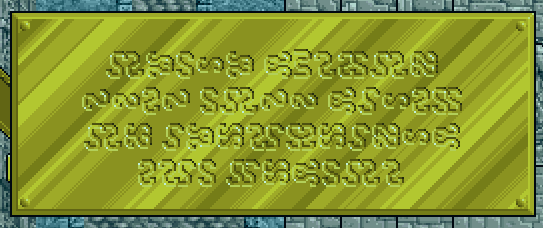
\includegraphics[scale=0.25]{ophidian-sign}
  \end{subfigure}
  
\end{figure}

\begin{figure}
  \centering
  \caption{}
  \begin{subfigure}{1\textwidth}
    \centering
    \caption{Encoding}
      \codepoint{E5E8} \codepoint{E5E5} \codepoint{E5E5} \codepoint{E5E7} \codepoint{E5E7} \codepoint{E5E5} \codepoint{E5E7} \codepoint{E5EF} \codepoint{E5ED} \codepoint{E5E5} \codepoint{E5E5} \codepoint{E5EA} \codepoint{E5ED} \codepoint{E5EF} \codepoint{E5FE} \codepoint{20} \codepoint{E5E5} \codepoint{E5E5} \codepoint{E5EE} \codepoint{20} \codepoint{E5E5} \codepoint{E5E5} \codepoint{E5ED} \codepoint{E5EF} \codepoint{20} \codepoint{E5E2} \codepoint{20}
      \codepoint{E5E5} \codepoint{E5E7} \codepoint{E5EF} \codepoint{E5ED} \codepoint{E5E4} \codepoint{E5E2} \codepoint{E5EE} \codepoint{20} \codepoint{E5E3} \codepoint{E5E3} \codepoint{E5E9} \codepoint{E5EB} \codepoint{E5ED} \codepoint{E5ED} \codepoint{E5EF} \codepoint{E5ED} \codepoint{E5EB} \codepoint{E5E9} \codepoint{E5E4} \codepoint{E5F1} \codepoint{20} \codepoint{E5EE} \codepoint{E5E9} \codepoint{E5EB} \codepoint{20}
      \codepoint{E5EB} \codepoint{E5EB} \codepoint{E5E5} \codepoint{E5E5} \codepoint{E5ED} \codepoint{E5EF} \codepoint{E5E5} \codepoint{E5E5} \codepoint{E5EE} \codepoint{20} \codepoint{E5EE} \codepoint{E5E6} \codepoint{E5E4} \codepoint{20} \codepoint{E5EE} \codepoint{E5E6} \codepoint{E5EF} \codepoint{E5ED} \codepoint{E5E4} \codepoint{E5E4} \codepoint{20}
      \codepoint{E5EE} \codepoint{E5E4} \codepoint{E5EA} \codepoint{E5E8} \codepoint{E5E7} \codepoint{E5E7} \codepoint{E5E4} \codepoint{E5ED} \codepoint{E5EF} \codepoint{20  } \codepoint{E5E9} \codepoint{E5EB} \codepoint{E5E7} \codepoint{E5E5} \codepoint{20} \codepoint{E5E9} \codepoint{E5EB} \codepoint{E5EF} \codepoint{E5ED} \codepoint{E5E0} \codepoint{E5E4} \codepoint{E5EF} \codepoint{E5ED} \codepoint{E5FF}

  \end{subfigure}
  
  \medskip
  
  \begin{subfigure}{0.32\textwidth}
    \centering
    \caption{Ophidian}
    \sampletext{
      \char"E5E8 \char"E5E5\char"E5E5\char"E5E7\char"E5E7\char"E5E5\char"E5E7\char"E5EF\char"E5ED\char"E5E5\char"E5E5\char"E5EA\char"E5ED\char"E5EF\char"E5FE\char"20\char"E5E5\char"E5E5\char"E5EE\char"20\char"E5E5\char"E5E5\char"E5ED\char"E5EF\char"20\char"E5E2\char"20\\
      \char"E5E5\char"E5E7\char"E5EF\char"E5ED\char"E5E4\char"E5E2\char"E5EE\char"20\char"E5E3\char"E5E3\char"E5E9\char"E5EB\char"E5ED\char"E5ED\char"E5EF\char"E5ED\char"E5EB\char"E5E9\char"E5E4\char"E5F1\char"20\char"E5EE\char"E5E9\char"E5EB\\
      \char"E5EB\char"E5EB\char"E5E5\char"E5E5\char"E5ED\char"E5EF\char"E5E5\char"E5E5\char"E5EE\char"20\char"E5EE\char"E5E6\char"E5E4\char"20\char"E5EE\char"E5E6\char"E5EF\char"E5ED\char"E5E4\char"E5E4\\
      \char"E5EE\char"E5E4\char"E5EA\char"E5E8\char"E5E7\char"E5E7\char"E5E4\char"E5ED\char"E5EF\char"20  \char"E5E9\char"E5EB\char"E5E7\char"E5E5\char"20 \char"E5E9\char"E5EB\char"E5EF\char"E5ED\char"E5E0\char"E5E4\char"E5EF\char"E5ED\char"E5FF\\
      
    }
  \end{subfigure}
  \begin{subfigure}{0.32\textwidth}
    \centering
    \caption{Latin}
    \sampletext{
      Pilgrims, it is a\\
      great journey to\\
      visit the three\\
      temples of order.\\
    }
  \end{subfigure}
  \begin{subfigure}{0.32\textwidth}
    \centering
    \caption{Screenshot}

    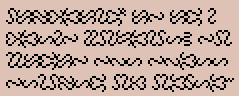
\includegraphics[scale=0.75]{ophidian-book}
  \end{subfigure}
  
\end{figure}

\section{Samples}



\end{document}
